\documentclass[aspectratio=169]{beamer}
\usepackage[T1]{fontenc}
\usepackage{multicol}
\usepackage{ragged2e}   %new code
\usepackage[utf8]{inputenc}
\usepackage[brazil]{varioref, babel}
\usepackage{xmpmulti}
\usepackage{epsfig}
\usepackage{caption}
\usepackage{subcaption}
\usepackage{siunitx}
\usepackage{mathtools}
\usepackage{amssymb}
\usepackage{amsmath}
\usepackage{booktabs}
\usepackage{pbox}
\usepackage{graphicx,url}
\usepackage{etoolbox}
\usepackage{ru,hyperref,url} % 
\graphicspath{{../figures/}}
\usepackage{indentfirst}

\usepackage{tikz}
\usetikzlibrary{shapes,arrows,fit, positioning, arrows.meta}
\usetikzlibrary{backgrounds}
\usepgflibrary{shapes.multipart}

\addtobeamertemplate{block begin}{}{\justifying}
\setbeamertemplate{section in toc}[sections numbered]
\setbeamersize{text margin left = 1em}
\setbeamertemplate{caption}[numbered]
\setbeamertemplate{bibliography item}[text]

\newcommand{\fmedida}{\text{F-medida }(\hat{y}(\mathbf{x}))}
\newcommand{\acuracia}{\text{Acurácia }(\hat{y}(\mathbf{x}))}
\newcommand{\sensibilidade}{\text{Sensibilidade }(\hat{y}(\mathbf{x}))}
\newcommand{\precisao}{\text{Precisão }(\hat{y}(\mathbf{x}))}

\newcommand{\doingles}[1]{\footnote{Do inglês: \emph{#1}.}}

% The title of the presentation:
%  - first a short version which is visible at the bottom of each slide;
%  - second the full title shown on the title slide;

\title{Detecção de doenças cardiovasculares através de sinais de ECG utilizando ferramentas de inteligência artificial}

% Optional: a subtitle to be dispalyed on the title slide
% \subtitle{Show where you're from}

% The author(s) of the presentation:
%  - again first a short version to be displayed at the bottom;
%  - next the full list of authors, which may include contact information;
\author[João Pedro O. Pagnan]{ \footnotesize
  Aluno: João Pedro de Oliveira Pagnan\\
  Professor: Prof. Dr. José Wilson Magalhães Bassani [CEB/UNICAMP]\\\medskip
  }

% The institute:
%  - to start the name of the university as displayed on the top of each slide
%    this can be adjusted such that you can also create a Dutch version
%  - next the institute information as displayed on the title slide
\institute[]{Universidade Estadual de Campinas - Faculdade de Engenharia Elétrica e Computação\\
  EA997 - Introdução à Engenharia Biomédica \\
  }

% Add a date and possibly the name of the event to the slides
%  - again first a short version to be shown at the bottom of each slide
%  - second the full date and event name for the title slide
\date{\scriptsize \today}

\renewcommand{\indent}{\hspace*{2em}}

\begin{document}

\setbeamertemplate{headline}{}
\setbeamertemplate{footline}{}

\begin{frame}
  \titlepage
\end{frame}

% Section titles are shown in at the top of the slides with the current section 
% highlighted. Note that the number of sections determines the size of the top 
% bar, and hence the university name and logo. If you do not add any sections 
% they will not be visible.
\section{Introdução}
\subsection{Identificação de doenças cardiovasculares com ferramentas de IA}
\begin{frame}
    \frametitle{Introdução}
    \justifying 
    \indent
    
    \indent{O diagnóstico de arritmias cardíacas através de sinais de eletrocardiograma (ECG) é de extrema importância para monitorar a saúde do coração através de um método não invasivo \cite{moody2001impact}. Devido a isso, uma boa etapa de interpretação de sinais computadorizados de ECG é fundamental para que o diagnóstico seja feito de forma precisa e, caso exista, a arritmia cardíaca seja detectada corretamente.}
    
    \indent{Embora que esta análise seja tradicionalmente feita por cardiologistas, trabalhos recentes indicam que ferramentas computacionais de aprendizado de máquina \doingles{Machine Learning} podem obter métricas de \textbf{f-medida} e \textbf{acurácia} melhores que as alcançadas por grande parte dos cardiologistas \cite{hannun2019cardiologist, rajpurkar2017cardiologist}.}
  
    \indent{Desta forma, estas ferramentas podem detectar diversos tipos de arritmias cardíacas a partir de uma única derivação com desempenho comparável ao de cardiologistas e, em contextos clínicos, podem reduzir a chance de diagnósticos incorretos e melhorar a interpretação do sinal de ECG de um especialista humano que já terá uma indicação da provável arritmia que o paciente possui \cite{rajpurkar2017cardiologist}.}    
    
\end{frame}

\begin{frame}
	\frametitle{Objetivos}
	\justifying
	
	\indent{Este projeto visa implementar e comparar quatro tipos de classificadores para identificar arritmias cardíacas através de sinais de ECG: um modelo baseado em máquinas de vetores-suporte (SVM\doingles{Support Vector-Machine}), outro baseado nos $k$ vizinhos mais próximos (KNN\doingles{K-Nearest Neighbors}), um terceiro baseado em florestas aleatórias (RF\doingles{Random Forest}) e, por fim, um baseado no tipo de rede neural LSTM \doingles{Long-Short Term Memory} \cite{geron2019hands}.}
	
	\indent{Neste caso, planeja-se também analisar qual a melhor representação para os sinais de ECG, isto é, se representaremos os sinais no domínio do tempo ou da frequência, bem como se o uso de filtros para remoção de ruído pode aprimorar o desempenho dos classificadores.}
\end{frame}

\begin{frame}
	\frametitle{Metodologia}
	\justifying

	\indent{Foi utilizada a linguagem \textbf{Python 3}, mais precisamente, as bibliotecas \textbf{Scikit-Learn} e \textbf{TensorFlow} e a base de dados\doingles{Dataset} aberta \textbf{MIT-BIH} \cite{moody2001impact}, que contém dados de 47 pessoas de 23 a 89 anos, incluindo homens e mulheres.}
	
	\indent{Esta base foi construída entre 1975 e 1979 e contém amostras de cinco padrões diferentes de batimento cardíaco: um padrão com o coração saudável, outro com bloqueio do ramo esquerdo, um terceiro com bloqueio do ramo direito, um quarto com contração atrial prematura e, por fim, um último com contração ventricular prematura. Estes padrões estão ilustrados na Figura \ref{fig:padroes-ECG}}.
	
	\indent{O dado foi digitalizado com uma frequência de $\SI{360}{\hertz}$ e cada sinal dura $\SI{1}{s}$, ou seja, cada sinal é um conjunto de $360$ valores e, por fim, foi utilizada a derivação precordial (V2).}
	
\end{frame}

\begin{frame}
	\frametitle{Metodologia}
	\justifying

	\vspace{25pt}

	\begin{figure}[H]
	\centering
	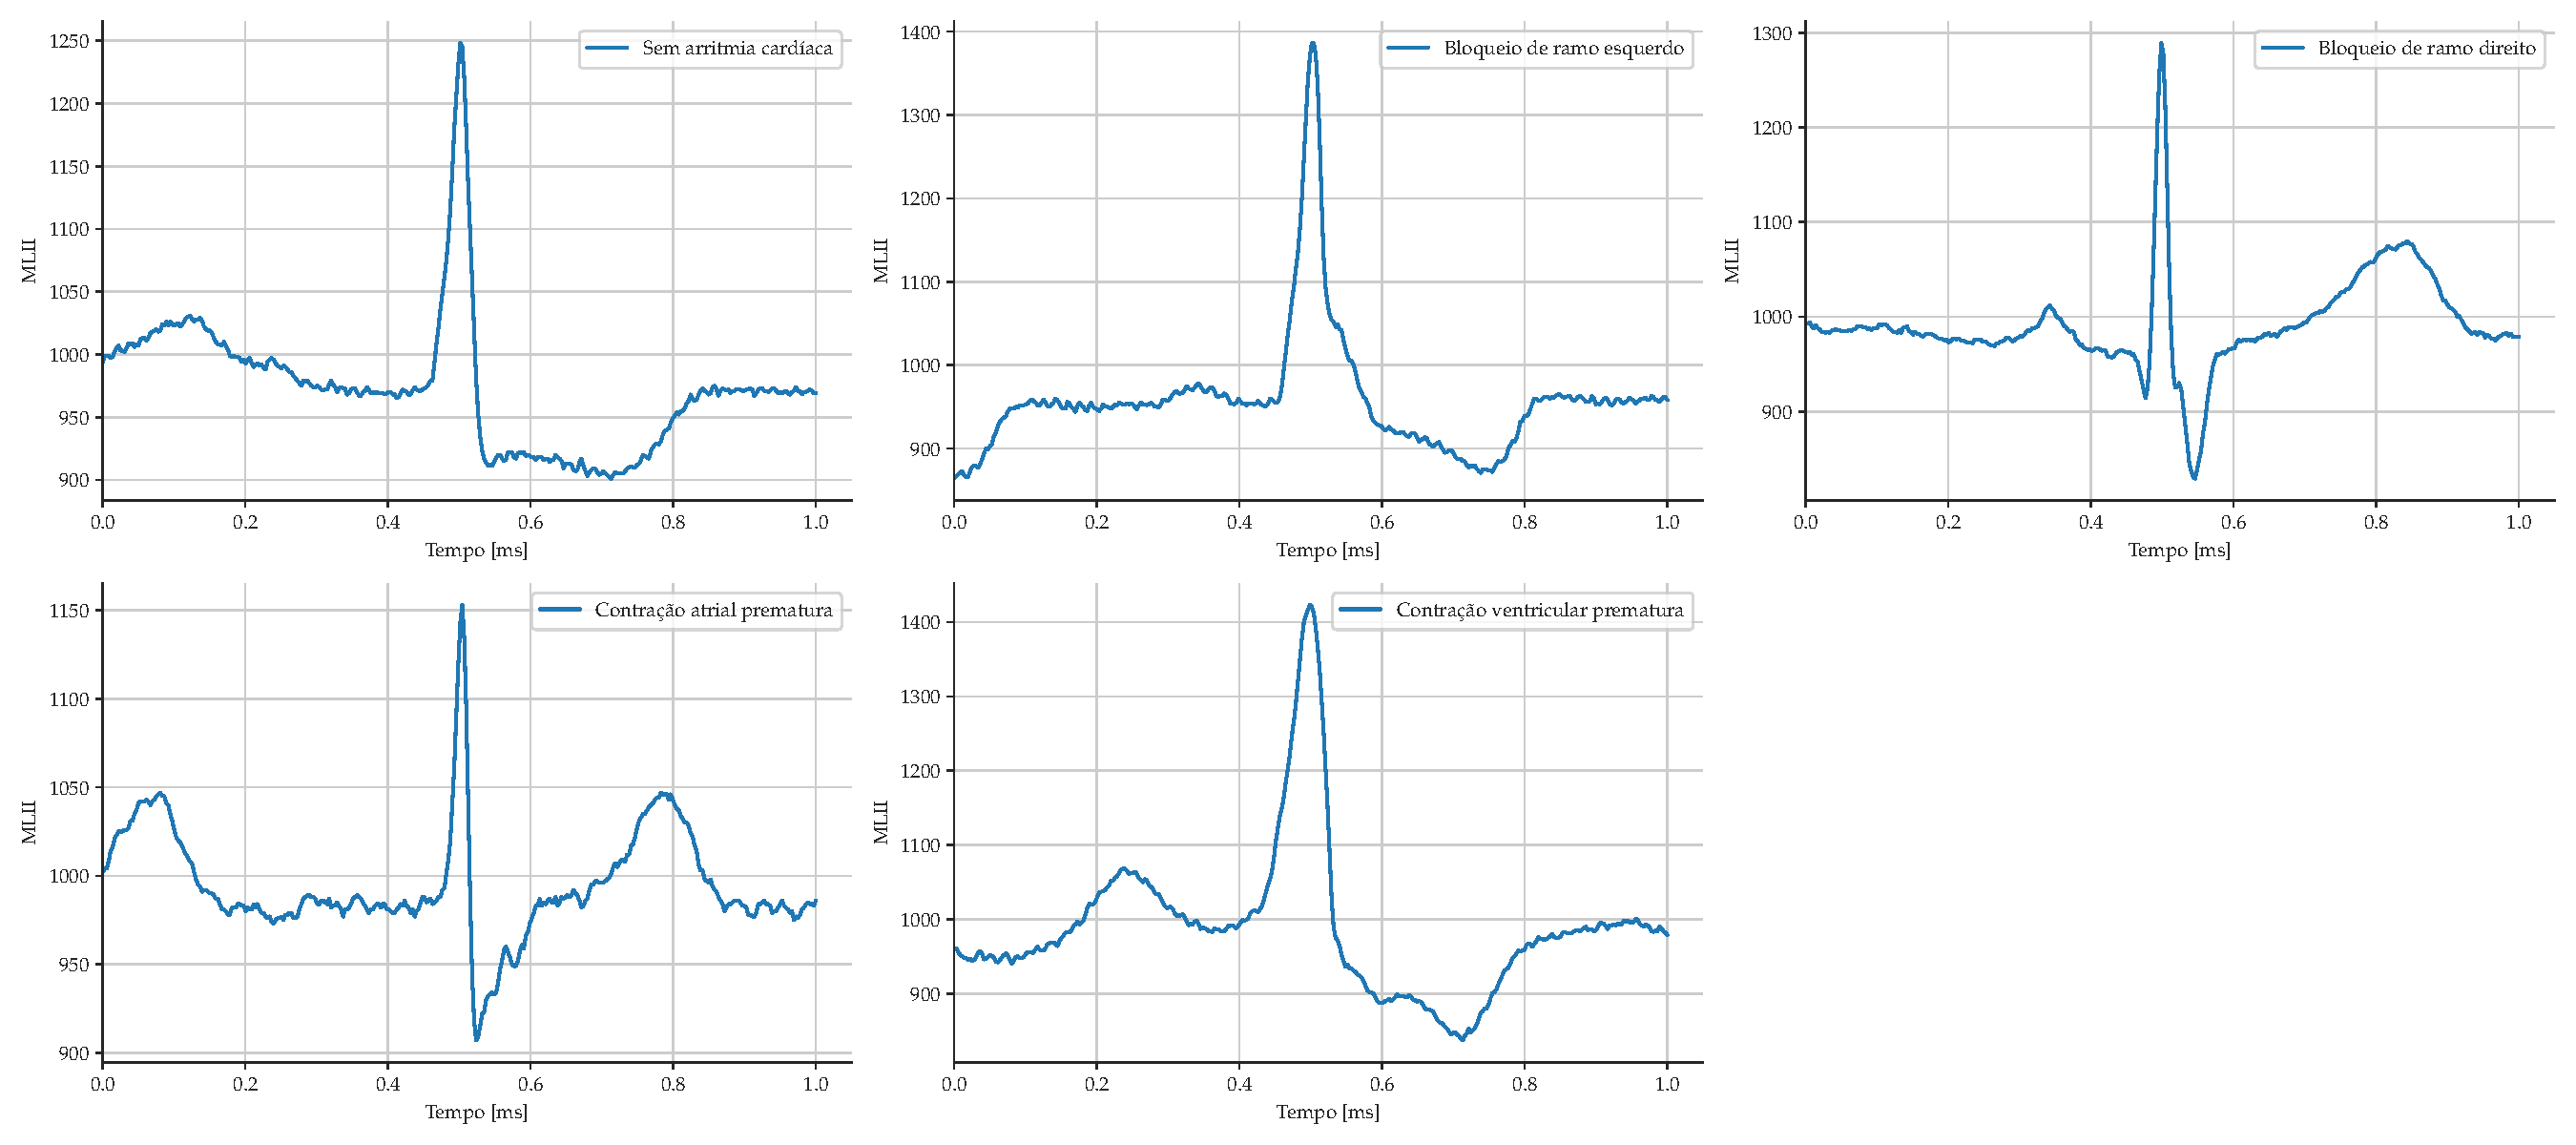
\includegraphics[scale = 0.2]{unfiltered-time-signals.pdf}
	\caption{Tipos de batimento cardíaco presentes nos sinais de ECG presentes na base de dados selecionada.}
	\label{fig:padroes-ECG}
	\end{figure}
	
	\indent{A base de dados foi balançeada para que todas as classes tenham a mesma proporção no conjunto final, ou seja, haja o mesmo número  de sinais (2546) em todos os tipos de batimentos cardíacos presentes nos sinais de ECG.}
\end{frame}	
	
\begin{frame}	
	\frametitle{Metodologia}
	\justifying
	
	\vspace{20pt}
	
	\indent{Após carregar as séries temporais, os dados foram normalizados utilizando a técnica \textit{z-score}, definida na equação (\ref{eq:z-score}).
	\begin{equation}\label{eq:z-score}
		x' = \frac{x - \mu}{\sigma},
	\end{equation}
	onde $x$ é o valor original, $x'$ é o valor normalizado, $\mu$ e a média dos valores do sinal e $\sigma$ é o desvio-padrão.}

\indent{Após este processo de normalização, foram criados os seguintes conjuntos de representações para os sinais:
\begin{enumerate}
	\item Séries temporais normalizadas;
	\item Séries temporais normalizadas e filtradas com um filtro passa-baixa;
	\item Módulos dos espectros de frequência das séries temporais normalizadas;
	\item Módulos dos espectros de frequência das séries temporais normalizadas e filtradas com um filtro passa-baixa;
\end{enumerate}}

\end{frame}

\begin{frame}
	\frametitle{Metodologia}
	\justifying

	\vspace{16pt}

	\indent{Com as representações, os modelos foram ajustados com base em um conjunto de treinamento que continha $75\%$ do número total de sinais e avaliados em um conjunto de teste composto por $25\%$ do total.}
	
	\indent{No caso da rede neural, como o ajuste dos pesos dos neurônios é iterativo, pois não há solução em forma fechada, o conjunto de treinamento possui $67.5\%$ do total de amostras para que haja um conjunto de validação composto por $7.5\%$ das coletas. Este conjunto será usado durante o treinamento da rede para evitar o problema do sobreajuste.}
	
	\indent{Para medir o desempenho dos modelos nesta tarefa, foram utilizadas as métricas numéricas de acurácia e f-medida definidas em (\ref{eq:metrics}):
\vspace{-8pt}
	
\begin{subequations}\label{eq:metrics}
	\scriptsize
		\begin{equation}
			\acuracia = \frac{TP + TN}{N},
		\end{equation}
	\begin{minipage}{0.5\textwidth}
		\begin{equation}
		\precisao = \frac{TP}{TP + FP},
		\end{equation}
	\end{minipage}
	\begin{minipage}{0.5\textwidth}
		\begin{equation}
			\sensibilidade = \frac{TP}{TP + FN},
		\end{equation}
	\end{minipage}
		\begin{equation}
			\fmedida = 2 \cdot \frac{\sensibilidade \cdot \precisao}{\sensibilidade + \precisao},
		\end{equation}
	\end{subequations}}

\vspace{-8pt}
sendo $N$ o total de amostras, $TP$ e $TN$ o número de verdadeiros positivos e negativos, respectivamente, e $FP$ e $FN$ o número de falsos positivos e negativos.

\end{frame}

\begin{frame}
	\frametitle{Resultados}
	\justifying

	\vspace{20pt}

	\indent{Utilizando as métricas indicadas anteriormente, foram obtidas as seguintes métricas para as representações utilizadas:}
	
	\begin{minipage}{0.5\textwidth}
	\tiny
	\begin{table}[H]
		\begin{center}
		\caption{Métricas obtidas para os sinais temporais não-filtrados.}
		\begin{tabular}{c c c c}
		\toprule
		\textbf{Modelo} & \textbf{Acurácia} & \textbf{F-medida} \\
		\midrule
		\textbf{SVM} & 0.9654 & 0.9658\\
		\textbf{KNN} & 0.9538 & 0.9541\\
		\textbf{RF} & 0.9627 & 0.9623\\
		\textbf{LSTM} & $(0.9709 \pm 0.0029)$ & $(0.9711 \pm 0.0029)$\\
		\bottomrule
		\end{tabular}
		\end{center}
	\end{table}
	\end{minipage}
	\hfill		
	\begin{minipage}{0.5\textwidth}
	\tiny
	\begin{table}[H]
		\begin{center}
		\caption{Métricas obtidas para os sinais temporais filtrados.}
		\begin{tabular}{c c c c}
		\toprule
		\textbf{Modelo} & \textbf{Acurácia} & \textbf{F-medida} \\
		\midrule
		\textbf{SVM} & 0.9544 & 0.9549\\
		\textbf{KNN} & 0.9560 & 0.95640\\
		\textbf{RF} & 0.9365 & 0.9372\\
		\textbf{LSTM} & $(0.9683 \pm 0.0041)$ & $(0.9685 \pm 0.0041)$\\
		\bottomrule
		\end{tabular}
		\end{center}
	\end{table}
	\end{minipage}
	
	\begin{minipage}{0.5\textwidth}
	\tiny
	\begin{table}[H]
		\begin{center}
		\caption{Métricas obtidas para os módulo dos espectros em frequência não-filtrados.}
		\begin{tabular}{c c c c}
		\toprule
		\textbf{Modelo} & \textbf{Acurácia} & \textbf{F-medida} \\
		\midrule
		\textbf{SVM} & 0.9061 & 0.9068\\
		\textbf{KNN} & 0.9538 & 0.9541\\
		\textbf{RF} & 0.9189 & 0.9189\\
		\textbf{LSTM} & $(0.9176 \pm 0.0066)$ & $(0.9190 \pm 0.0067)$\\
		\bottomrule
		\end{tabular}
		\end{center}
	\end{table}
	\end{minipage}
	\hfill
	\begin{minipage}{0.5\textwidth}
	\tiny
	\begin{table}[H]
		\begin{center}
		\caption{Métricas obtidas para os módulo dos espectros em frequência filtrados.}
		\begin{tabular}{c c c c}
		\toprule
		\textbf{Modelo} & \textbf{Acurácia} & \textbf{F-medida} \\
		\midrule
		\textbf{SVM} & 0.8960 & 0.8966\\
		\textbf{KNN} & 0.9010 & 0.9013\\
		\textbf{RF} & 0.9139 & 0.9139\\
		\textbf{LSTM} & $(0.9247 \pm 0.0037)$ & $(0.9253 \pm 0.0039)$\\
		\bottomrule
		\end{tabular}
		\end{center}
	\end{table}
	\end{minipage}
	
\end{frame}

\begin{frame}
	\frametitle{Resultados}
	\justifying
	
	\vspace{17pt}

	\indent{Utilizando a representação que obteve os melhores valores para as métrica (sinais temporais não-filtrados) foram obtidas as  matrizes de confusão indicadas na Figura \ref{fig:conf-matrix} para os classificadores utilizados:}
	
	\begin{figure}[H]
		\begin{subfigure}[H]{0.325\textwidth}
			\centering
			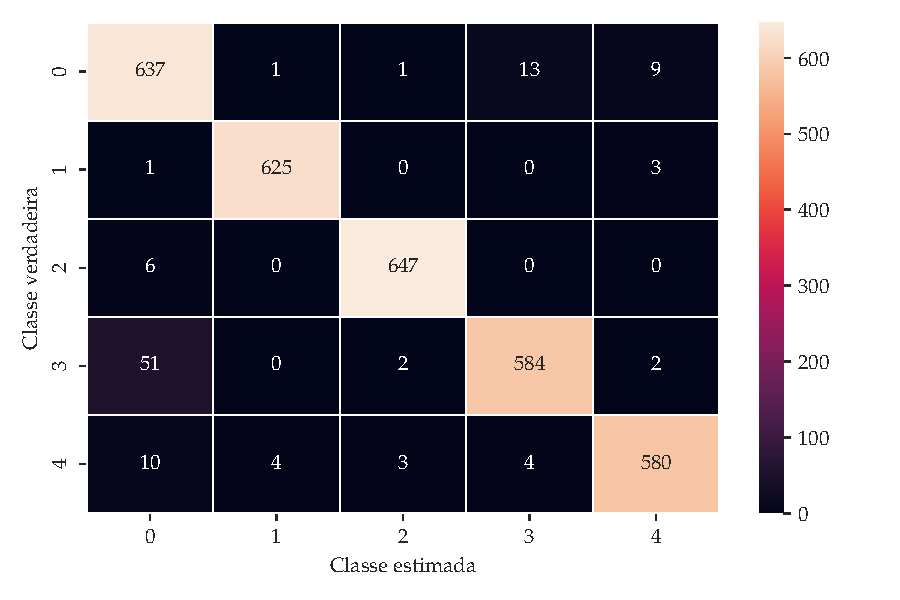
\includegraphics[scale=0.2]{svm-confusion-matrix}
			\caption{\scriptsize SVM}
		\end{subfigure}
		\centering
		\begin{subfigure}[H]{0.325\textwidth}
			\centering
			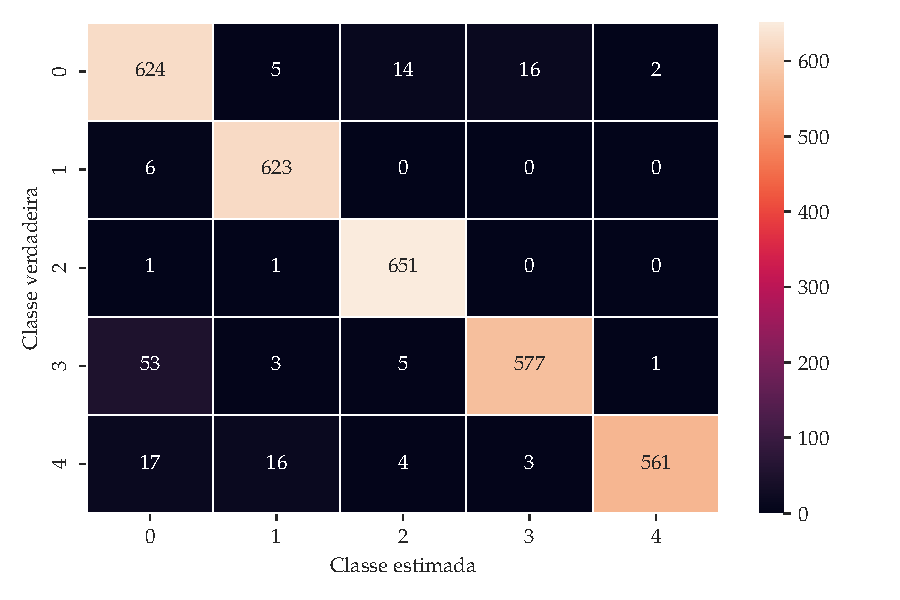
\includegraphics[scale=0.2]{knn-confusion-matrix}
			\caption{KNN}
		\end{subfigure}
		\\
		\centering
		\begin{subfigure}[H]{0.325\textwidth}
			\centering
			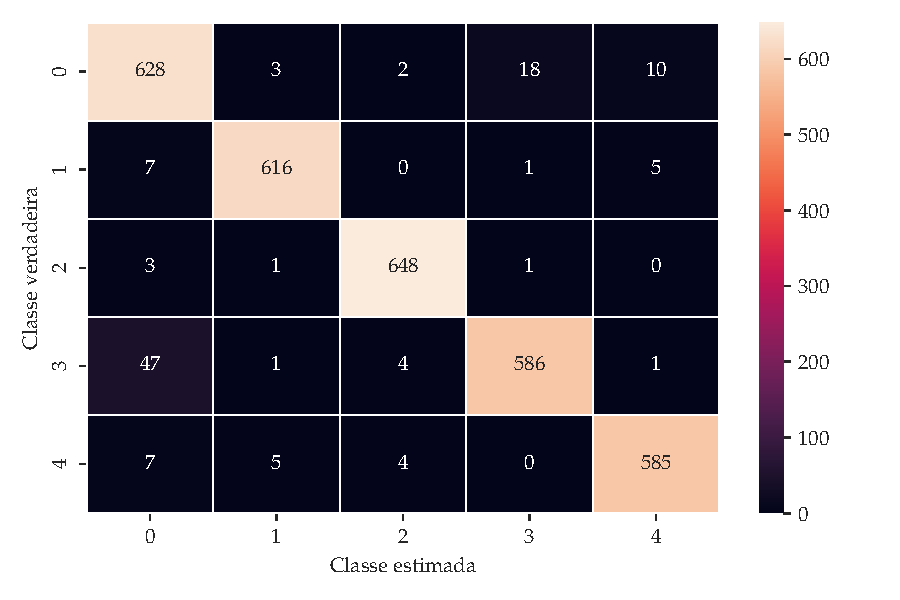
\includegraphics[scale=0.2]{rf-confusion-matrix}
			\caption{RF}
		\end{subfigure}
		\centering
		\begin{subfigure}[H]{0.325\textwidth}
			\centering
			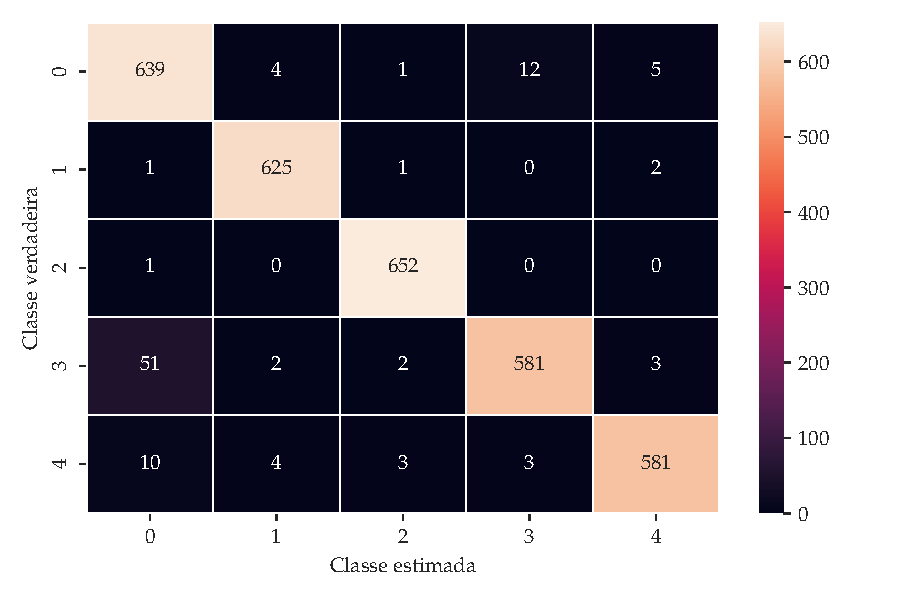
\includegraphics[scale=0.2]{lstm-confusion-matrix}
			\caption{LSTM}
		\end{subfigure}
		\centering
		\caption{Matrizes de confusão obtidas pelos quatro modelos avaliados utilizando os sinais temporais não-filtrados.}
		\label{fig:conf-matrix}
	\end{figure}		
	
\end{frame}

\begin{frame}
	\frametitle{Discussão}
	\justifying

	\vspace{15pt}	
	
	\indent{Analisando os resultados obtidos pode-se perceber que:
	\begin{enumerate}
		\item Representar os dados de ECG no formato de séries temporais favorece a classificação;
		\item A filtragem utilizada prejudicou a classificação;
		\item O melhor modelo classificador (em todas as representações) foi o baseado em redes LSTM;
		\item A classificação incorreta que mais prejudicou o desempenho de todos os modelos foi a confusão da classe 0 com a classe 3, ou seja, os classificadores indicaram que um sinal de ECG de uma pessoa com contração atrial prematura é o de uma pessoa com coração saudável.
	
	\vspace{10pt}
	
	\indent{Devido ao quarto ponto mencionado acima, recomenda-se que, caso seja determinado pelo modelo que o indivíduo não possui as arritmias analisadas, esta pessoa faça mais exames para confirmar este fato.}
	
	\end{enumerate}}
\end{frame}

\begin{frame}
	\frametitle{Conclusão}
	\justifying
	
	\indent{Com este projeto conclui-se que ferramentas de aprendizado de máquina podem ser bem úteis para a análise clínica de sinais de ECG coletadas de pacientes.}
	
	\indent{Obviamente, esta é uma análise preliminar feita com apenas quatro tipos de arritmia (além de sinais de corações saudáveis), mas, junto a outros trabalhos da literatura, como \cite{moody2001impact, hannun2019cardiologist} e \cite{rajpurkar2017cardiologist}, é um bom indicador de que este tipo de ferramenta tem espaço em análises médicas.}
	
	\indent{Mais precisamente, ferramentas baseadas em aprendizado de máquina para classificar sinais de eletrocardiograma seriam bem utilizadas em regiões do país (e do mundo) onde não há cardiologistas suficientes para atenderem à demanda das populações locais.}
	
	\indent{Desta forma, conclui-se que este projeto cumpriu o seu propósito de detecção de doenças cardiovasculares através de sinais e ECG utilizando ferramentas de inteligência artificial.}	
	
\end{frame}

\appendix

\begin{frame}{Referências}
    \tiny
    \bibliography{bib}
    \bibliographystyle{ieeetr}
\end{frame}

\begin{frame}[plain,c]
    \begin{center}
    \Huge Muito Obrigado!
    \end{center}
\end{frame}


\end{document}
